\documentclass[11pt,thesis]{starthesis} %use twoside option for book printing
%\documentclass[11pt, twoside, MSc]{starthesis}
\usepackage[round]{natbib}
\usepackage{aas_macros}
\usepackage{times}
\usepackage{lscape}
\usepackage{amssymb}
%\usepackage{psfig,epsfig,dcolumn}
\usepackage{times}
\usepackage[utf8]{inputenc}
\usepackage{amssymb}
\usepackage{epsf}
\setcounter{secnumdepth}{3}
%\usepackage{rotating}
\usepackage{multirow}
\usepackage[toc,page]{appendix}
\usepackage{placeins}
\usepackage{epsfig}
%\usepackage{subfigure}
\usepackage{makeidx}
\usepackage{url}
\usepackage[margin=1cm,labelfont=bf,font={small}]{caption}
\usepackage{fancyhdr}
\usepackage[headsep=0.5cm,headheight=3cm]{geometry}
\usepackage{sectsty}
\usepackage{longtable}
\usepackage{caption}
\usepackage{enumitem}
\usepackage{titlesec}
\usepackage{array}
\usepackage{longtable}

% MGL PACKAGES
\usepackage{gensymb} % Allows degrees symbol
\usepackage{graphicx}	% Including figure files
\usepackage{amsmath}	% Advanced maths commands
\usepackage{booktabs}   % Gives nicer formatting for Table 2
\usepackage{cuted}      % Used to display the large matrix in the appendix across two columns
\usepackage{upgreek}    % gives a nicer looking \mu symbol than the default, to represent "micro" as a prefix
\usepackage{hyperref}   % allows URL hyperlinks to publicly-available source code
\hypersetup{
    colorlinks,
    linkcolor={red!0!black},
    citecolor={blue!80!black},
    urlcolor={blue!80!black}
}
% \usepackage{amssymb}	% Extra maths symbols
\usepackage{xcolor}     % Allows colors for highlighting changes in response to reviewer comments
\usepackage[normalem]{ulem}       % Allows strikethrough for highlighting changes in response to reviewer comments
\usepackage{braket}     % Allows <bra-ket> notation for cos(theta) terms
\usepackage{subcaption}     % Allows <bra-ket> notation for cos(theta) terms
\usepackage[version=4]{mhchem} % Does all the subscripts for you in chemical equations (e.g. just write \ce{Mg2SiO4})
\usepackage{adjustbox}
\usepackage{changepage}

\makeindex
\fancyhf{}

\def\gappeq{\mathrel{ \rlap{\raise.5ex\hbox{$>$}}
                      {\lower.5ex\hbox{$\sim$}}  } }
\def\lappeq{\mathrel{ \rlap{\raise.5ex\hbox{$<$}}
                      {\lower.5ex\hbox{$\sim$}}  } }

\makeatletter
\renewcommand{\@chapapp }{}
\makeatother

\newcommand{\revise}[1]{\textcolor{red}{\bf#1}}

\chapternumberfont{\fontsize{60}{70}\selectfont}
\chaptertitlefont{\fontsize{20}{20}\selectfont}

\begin{document}
\title{My Thesis Title}

\author{Your Name}
\dept{Physics}     
\principaladviser{Prof. Xavier and Dr. Who}
\submitdate{December 2026}
\copyrightyear{2026}
\copyrightfalse
\sigpagefalse 
%\beforeabstract
%\afterabstract
\pagestyle{plain}
\include{dedication}
%\afterpreface
\pagestyle{plain}

\hsp
% Define these variables.
\title{My Thesis Title}
\author{Author}

\submitdate{December 2026}
\copyrightyear{2026}
\dept{Physics}     
\principaladviser{Prof. Xavier and Dr. Who} 

\pagenumbering{roman} % Jan 2000 GSAS Harvard req.
\pagestyle{empty}
\titlep % see starthesis.cls

%\sigpagefalse 
%\beforeabstract
%\afterabstract

%%%%%%%%%%%%%%%%%%%%%% Synopsis %%%%%%%%%%%%%%%%%%%%%%%%%%%%%%%%%%%%%
\cleardoublepage
\pagestyle{plain} 
\section*{Abstract}

Science is very important. Bla bla bla.

%%%%%%%%%%%%%%%%%%%%% Dedication %%%%%%%%%%%%%%%%%%%%%%%%%%%%%%%%

\cleardoublepage
\pagestyle{plain} 
\section*{Dedication (Optional)}
    \vspace{0.25\textheight}
    \begin{center}
        \textit{To Warner Hunnington III. \\ I'll show you how valuable Elle Woods can be.}
    \end{center}


%%%%%%%%%%%%%%%%%%%%% Acknowledgments %%%%%%%%%%%%%%%%%%%%%%%%%%%%%%%%

\cleardoublepage
\pagestyle{plain} 
\section*{Acknowledgements (Optional)}

I did it all by myself.

Last but not least, I wanna thank me. I wanna thank me for believing in me. I wanna thank me for doing all this hard work. I wanna thank me for having no days off. I wanna thank me for never quitting.

%%%%%%%%%%%%%%%%%%%% DECLARATION  %%%%%%%%%%%%%%%%%%%%%%%%%%%%%%%%%%%%%
\cleardoublepage
\phantomsection
\pagestyle{plain} 
\begin{declaration}

I declare that the work in this dissertation was carried out in accordance with the requirements of the University's Regulations and Code of Practice for Research Degree Programmes and that it has not been submitted for any other academic award. Except where indicated by specific reference in the text, the work is my own work. Work done in collaboration with, or with the assistance of, others is indicated as such. I confirm that I have read, and that this work complies with, the University’s guidance for PGR students on the use of artificial intelligence tools in thesis writing. Any views expressed in the dissertation are those of the author.

\par\vspace*{3cm}\par

\noindent SIGNED: Your Name. \\ 
DATE: 01/12/26

%\vspace{2cm}

\end{declaration}

%%%%%%%%%%%%%%%%%%%% STATEMENT ON THE INCLUSION OF PUBLISHED AND COLLABORATIVE WORK  %%%%%%%%%%%%%%%%%%%%%%%%%%%%%%%%%%%%%
\cleardoublepage
\phantomsection
\pagestyle{plain} 
\begin{statement_published_work}

My dissertation does include work that has been published, submitted or prepared for publication with me as an author.
My dissertation does not include non-published collaborative work that contains data or contributions from others.

\noindent If there are any publications with me as an author and/or any collaborative work that contains data or contributions from others, I have completed the following table. 

% MGL CUSTOM LONGTABLE (spans across separate pages)

% make custom column command to left-align text
\newcolumntype{L}[1]{>{\raggedright\arraybackslash}p{#1}}

% custom command for making space between paragraphs within longtable environment
\newcommand{\blankline}{\par\vspace{1em}}

\begin{longtable}{L{0.2\linewidth} | L{0.45\linewidth} | L{0.35\linewidth}}

    \hline
    \textbf{Chapter}  & \textbf{Publication or collaboration details} & \textbf{Author contributions}\\
    %The chapter or section that contains the student’s own published work or collaborative work. Specify if this forms a whole chapter, a whole section, or has been included in smaller segments 
    %& Details on the publication, including title of the work, author list, name of journal or preprint service, and weblink to the publication (if available) OR an overview of how the collaboration was conducted.
    %& Details on the specific contributions of each author to the publication or of each contributor to the collaboration. \\
    \hline
    \endfirsthead

    % this part does the running head for the column titles on subsequent pages
    \hline
    \textbf{Chapter}  & \textbf{Publication or collaboration details} & \textbf{Author contributions}\\
    \hline
    \endhead
    
    Chapter 1: Introduction 
    & Parts from the introductions of each of the following published papers were combined to make the introduction of the thesis. This is to enhance readability and prevent repetition of the context at the start of each chapter: 
    \blankline
    \textit{“Aerosols are not Spherical Cows: Using Discrete Dipole Approximation to Model the Properties of Fractal Particles” (2024)}
    \par
    Lodge, M., Wakeford, H. and Leinhardt, Z., MNRAS, 527(4), pp.11113-11137
    
    & All of this section is written entirely by me, including integration of a small amount of content from the introductions from my published papers.
    \\
    \hline
    
    Chapter 2: Theoretical Methods 
    & The theory sections of the following papers have been extracted into their own chapter, to prevent repetition:
    \blankline
    \textit{“Aerosols are not Spherical Cows: Using Discrete Dipole Approximation to Model the Properties of Fractal Particles” (2024)} 
    \par
    Lodge, M., Wakeford, H. and Leinhardt, Z., MNRAS, 527(4), pp.11113-11137.
    \blankline
    & These explanations are identical to those written by me in the published papers, with the one exception that small typos in the original DDA-FCD equations have been corrected here.
    \\
    \hline
    
    Chapter 3: A Science Chapter
    & All sections of this chapter were published as a journal article:
    \blankline
    \textit{“Aerosols are not Spherical Cows: Using Discrete Dipole Approximation to Model the Properties of Fractal Particles” (2024)}
    \par
    Lodge, M., Wakeford, H. and Leinhardt, Z., MNRAS, 527(4), pp.11113-11137.
    \blankline
    The published journal article was slightly modified for this chapter by merging the appendices into the main text.  
    & I wrote all code, prepared the publication and created all figures used. Other co-authors provided valuable guidance and diagnostic expertise in advisory and supportive roles.
    \\
    \hline
    
    Chapter 8: Extended Discussion 
    & This section was not published, and was entirely new for the thesis.
    & Entirely written by me.
    \\
    \hline
    
    Chapter 9: Conclusions 
    & This section was not published, and was entirely new for the thesis.
    & Entirely written by me.
    \\    
    \hline

\end{longtable}

The information in this table counts as the references to my own publications if they are used as whole chapters or as whole sections of chapters. If work from my own publications has been incorporated in smaller segments, I have included individual references to them in the relevant part of the dissertation in addition to completing the table.

%\vspace{2cm}

\end{statement_published_work}


%%%%%%%%%%%%%%%%%%%%% Table of contents etc  %%%%%%%%%%%%%%%%%%%%%%%%%
\cleardoublepage
\phantomsection
\addcontentsline{toc}{section}{Table of Contents}
\thispagestyle{empty}
\tableofcontents

\pagestyle{plain}

\cleardoublepage
\phantomsection
\addcontentsline{toc}{section}{List of Figures}
\thispagestyle{empty}
\listoffigures


\cleardoublepage
\phantomsection
\addcontentsline{toc}{section}{List of Tables}
\thispagestyle{empty}
\listoftables

% ADD LIST OF ABBREVIATIONS
\cleardoublepage
\phantomsection
\addcontentsline{toc}{section}{List of Abbreviations}
\thispagestyle{plain}
\chapter*{List of Abbreviations}

% define new column types
\newcolumntype{C}[1]{>{\centering\bfseries\arraybackslash}p{#1}} % centered, bold
\newcolumntype{B}[1]{>{\raggedright\bfseries\arraybackslash}p{#1}} % centered, bold
\newcolumntype{L}[1]{>{\raggedright\arraybackslash}p{#1}}       % left-aligned

\begin{longtable}{@{} B{0.25\textwidth} L{0.7\textwidth} @{}} % 25% the acronym, 75% the full version

    AAA & All Acronyms Alphabetical \\
    HPC & High-Performance Computing \\
    HST & Hubble Space Telescope \\
    ISM & Interstellar Medium \\
    JWST & James Webb Space Telescope \\
    SEM & Scanning Electron Microscope \\
    SNR & Signal-to-noise ratio \\
    STIS & Space Telescope Imaging Spectrograph \\
    TEM & Transmission Electron Microscope \\
    VTPR & Very Tired Postgraduate Researcher \\
    YMCA & Young Men's Christian Association \\
    ZZZ & ZStudent ZWithout ZCoffee

\end{longtable}


\cleardoublepage

\startarabicpagination % switch from roman numerals to numbers

\pagestyle{fancy}
\fancyhf{}
\fancyhead[LE]{\it\nouppercase\leftmark\slshape}
\fancyhead[RO]{\it\nouppercase\rightmark\slshape}
\fancyfoot[C]{\thepage}
\renewcommand{\headrulewidth}{0.4pt}
\renewcommand{\footrulewidth}{0pt}

\cleardoublepage
\chapter{Introduction}\label{chapter:introduction}

\section{First Section of My Introduction}

\subsection{Key Motivations for this Research}
Finding any motivation to conduct research is left as an exercise for the reader.

Say some things and cite some things.

\texttt{Astropy} is helpful astronomy software \citep{astropy2022}.

\begin{figure}
    \centering
	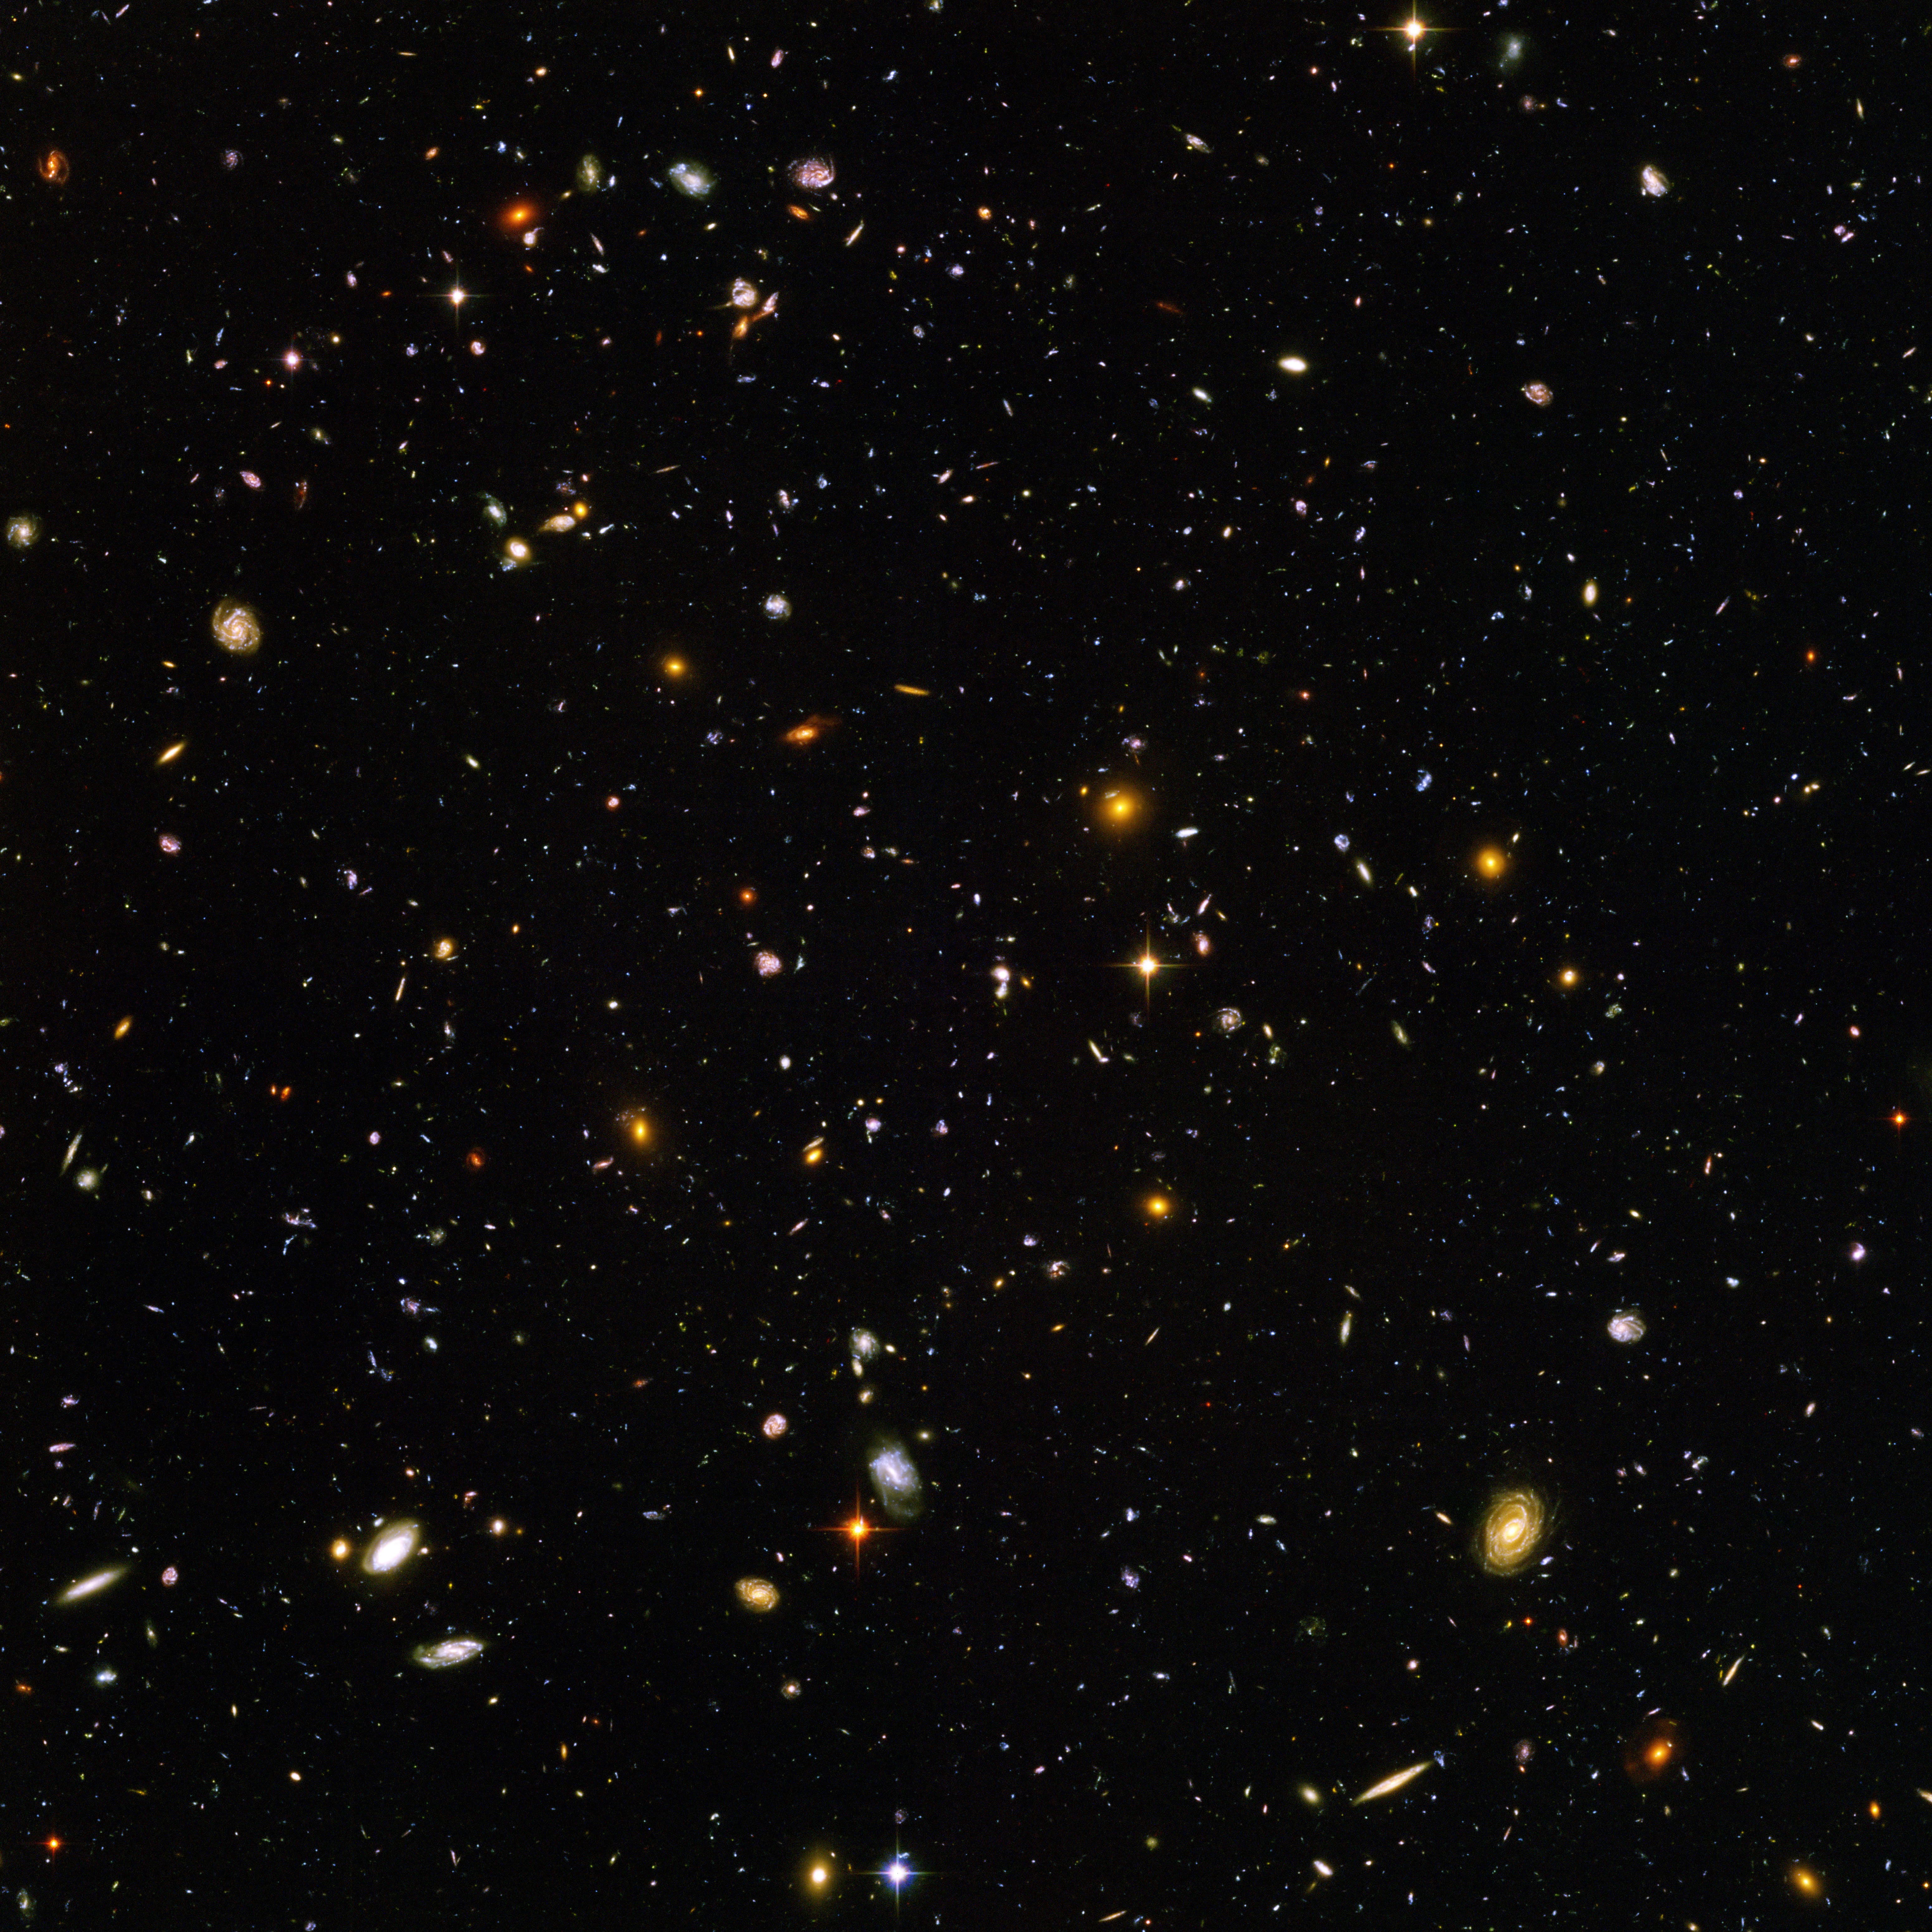
\includegraphics[width=13cm]{Images/Hubble_ultra_deep_field_high.jpg}
    \caption[Hubble ultra-deep field. (short name for list of figures)]{Hubble Ultra-Deep Field, in the constellation Fornax, 2004. Used with permission from NASA and the European Space Agency. Public Domain, https://commons.wikimedia.org/w/index.php?curid=5276968}
    \label{fig:hubble_deep_field}
\end{figure}

Detecting exoplanets itself has been a major recent scientific achievement, but with their existence confirmed, many studies have now moved their focus to attempting to characterize them. We can broadly assign categories (e.g. small rocky planets, hot Jupiters, water worlds) and carry out population-level studies to determine how frequently each type occurs.

\subsection{Etc}

More about your science.

\section{Thesis Structure}

The remainder of this thesis is structured as follows. Chapter~\ref{chapter:methods} introduces methods of science -- the methods introduced here are fundamental across several other Chapters. Chapter~\ref{chapter:science1} explores science. Chapter \ref{chapter:science2} presents even more science. In Chapter~\ref{chapter:science3} -- who would have guessed -- there is even more even more science. Finally, Chapter~\ref{chapter:conclusions} reflects on the thesis as a whole and concludes.
\chapter{Methods}
\label{chapter:methods}

\begin{center}
    \textit{This Chapter is adapted from work published somewhere, which summarises some science.}
\end{center}

To do science, we need methods. However, scientists tend to simply ``skim'' the methods section of a paper.

\section{The Socratic Method}
Write about your methods here.

\chapter{Science Chapter: First One}
\label{chapter:science1}

\begin{center}
    \textit{This chapter is adapted from work published in (cite your paper).}
\end{center}

\section{Introduction}
What happens in science chapter 1?

\section{Etc}
More chapter.
\chapter{Science Chapter: Second One}
\label{chapter:science2}

\begin{center}
    \textit{This chapter is adapted from work published in (cite your paper).}
\end{center}

\section{Introduction}
What happens in science chapter 2?

\section{Etc}
More chapter.
\chapter{Science Chapter: Third One}
\label{chapter:science3}

\begin{center}
    \textit{This chapter is adapted from work published in (cite your paper).}
\end{center}

\section{Introduction}
What happens in science chapter 3?

\section{Etc}
There is a table in this chapter.

\begin{table}
    \centering
    \begin{tabular}{cccccc} % eight columns, alignment for each
        \hline \vspace{-1em} \\
	{$N$} & $h_{\rm max}$ ($\rm R_{\oplus}$) & $\rho_{\rm min}$ ($\rm{kg \ m^{-3}}$) & $R_t = R_i$ ($\rm R_{\oplus}$) & $M_t = M_i$ ($\rm M_{ \oplus}$) & $v_c = v_{\rm esc}$ \\
    
    \hline \vspace{-0.75em}
    \\
    $10^5$ & 1 & $8.58 \times 10^{-2}$ & 0.970 & 0.897 & 10.757 \\
    $10^5$ & 2 & $1.07 \times 10^{-2}$ & 0.970 & 0.897 & 10.757 \\
    $10^5$ & 3.162 & $2.71 \times 10^{-3}$ & 0.970 & 0.897 & 10.757 \\
    
    % \hline
    \vspace{-0.5em} \\ 
	$10^6$ & 0.316 & $2.73 \times 10^{-1}$ & 0.983 & 0.897 & 10.685 \\
    $10^6$ & 1 & $8.62 \times 10^{-3}$ & 0.983 & 0.897 & 10.685 \\
    $10^6$ & 2 & $1.08 \times 10^{-3}$ & 0.983 & 0.897 & 10.685 \\
    $10^6$ & 3.162 & $2.73 \times 10^{-4}$ & 0.983 & 0.897 & 10.685  \\
    
    
    \\ \hline \hline
    \end{tabular}
    \caption[Table Name in List of Tables]{This table shows some data.}
    \label{tab:data}
\end{table}
\chapter{Conclusions}
\label{chapter:conclusions}

This thesis aimed to terminate my postgraduate studies. 

\section{Important Conclusion}
PhD degrees involve scientific research.

\section{Another Important Conclusion}
Scientific research is painful.

\section{Final Conclusions}
PhD degrees are painful.
\pagestyle{plain}
\cleardoublepage
\appendix
\pagestyle{fancy}
\chapter{Some Extra Stuff}
\label{chapter:appendixa}

\begin{center}
    \textit{Adapted from work published in (cite your paper).}
\end{center}

Extra, read all about it.
\chapter{More Extra Stuff}
\label{chapter:appendixa}

\begin{center}
    \textit{Adapted from work published in (cite your paper).}
\end{center}

Extra, extra, read all about it.
\printindex
\dsp
\addcontentsline{toc}{chapter}{Bibliography}
\bibliographystyle{mnras}
\bibliography{references}

\end{document}
